\documentclass[12pt,a4paper]{article}
\usepackage[utf8]{inputenc}
\usepackage[croatian]{babel} % For Croatian 
\usepackage[T1]{fontenc} % Better hyphenation for words with digraphs čćžšđ
\usepackage{graphicx}
\usepackage{color}
\usepackage{float} % For manualy figure postioning
\usepackage{listings} % Support for .txt listings w/o begin{verbatim}
\usepackage[usenames,dvipsnames]{xcolor} % Enabling more defined colors
\usepackage{datetime}
\usepackage{tocloft} % For Toc with dots
\usepackage[left=2.5cm,top=2.5cm,right=2cm,bottom=2.5cm]{geometry} 
\usepackage{fancyhdr} % For fancy headers and footers
\usepackage[nottoc]{tocbibind} % For adding Bibliography in TOC
\usepackage{amsmath}
\usepackage{listings}
\usepackage{setspace}
\usepackage{pdfpages}

% Fancy header definition
\pagestyle{fancy}
\renewcommand{\headrulewidth}{0pt} % Removes default rule in header
\fancyhf{}
% Set page number in down-right corner of the page
\rfoot{\thepage}

\begin{document}

% Section, figure, table numbering
\renewcommand{\thesection}{\arabic{section}.}
\renewcommand{\thesubsection}{\arabic{section}.\arabic{subsection}}
\renewcommand{\thefigure}{\arabic{section}.\arabic{figure}} 
\renewcommand{\thetable}{\arabic{section}.\arabic{table}}

\newpage
\begin{titlepage}
\begin{center}

\textbf{\MakeUppercase{\large 
    Sveučilište Josipa Jurja Strossmayera u Osijeku}}\\[0.2cm]

\textbf{\MakeUppercase{\large Elektrotehnički fakultet}}\\[0.8cm]
\textbf{\large Sveučilišni studij}\\ [5cm]

\textbf{\MakeUppercase{\Large 
    Izgradnja 3D modela scene pomoću 3D kamere }}\\ [1cm]

\textbf{\large Diplomski rad}\\  [5 cm] 

\textbf{\Large Marijan Svalina}\\ [0.5cm] 

\vfill

\textbf{\large Osijek, 2013.} \\

\end{center}
\end{titlepage}

% \includepdf[pages={1}]{Obrazac_Z1_04.pdf}
% \includepdf[pages={1}]{izjava_o_originalnosti}
\newpage
% Toc  
\renewcommand{\cftsecleader}{\cftdotfill{\cftdotsep}}
\tableofcontents 
% Removing page numbering from this page 
\thispagestyle{empty}

\newpage

\setcounter{page}{1}
\setcounter{figure}{0}
\section{Uvod}% (fold)
\label{sec:Uvod}

\subsubsection{Zadatak diplomskog rada} % (fold)
\label{ssub:Zadatak diplomskog rada}

Program RGBDSLAM raspoloživ u okviru programske biblioteke OpenSLAM
omogućava izgradnju 3D modela objekata i scena pomoću 3D kamere.
Razviti program za izgradnju 3D modela u obliku mreže trokuta koristeći
biblioteku PointCloud. Kombinacijom ova dva programa mogu se izgraditi
3D modeli objekata i scena snimljenih iz više pogleda. Zadatak je
ispitati funkcionalnost navedenog postupka kao i kvalitetu dobivenog
rezultata izgradnjom nekoliko 3D modela objekata i scena.

% subsubsection Zadatak diplomskog rada (end)
% section Uvod (end)

\newpage

\section{Teorija} % (fold)
\label{sec:Teorija}

Ovdje cu pisati o matematici iza istovremene lokalazacije i mapiranja.
Te o rekonstrukciji površina objekata i scene pomoću triangulacije.


\subsection{SLAM} % (fold)
\label{sub:SLAM}

\subsection{Triangulacija} % (fold)
\label{sub:Triangulacija}

% subsection Triangulacija (end)
% subsection SLAM (end)
% section Teorija (end)

\include{05-program-description}
\newpage
\setcounter{figure}{0}

\section{Rezultati} % (fold)
\label{sec:Rezultati}

Tijekom izrade diplomskog rada snimljeno je šest scena upotrebom
programa RGBDSlam i iz tih snimaka (slika~\ref{fig:01-all.png}) su
izgrađeni 3D modeli objekata i scena pomoću programa
\texttt{mesh-reconstruction}. Sve snimke i izrađeni modeli nalaze se na
priloženom DVDu. U ovom poglavlju su prikazani rezultati izgradnje i
ispitana je funkcionalnost izgradnje 3D modela scena pomoću 3D kamere.
Za ispitivanje funkcionalnosti metode odabrane su tri scene:
etfos-ured-2013-07-30, etfos-hol-2013-11-20, etfos-hodnik-11-27. Prije
prikaza rezultata potrebno je istaknuti nekoliko problema odnosno
ograničenja ove metode.

Problemi sa načinom stjecanja oblaka točaka
Problemi sa izgradnjom 3D modela 

\begin{figure}[h]
\centering
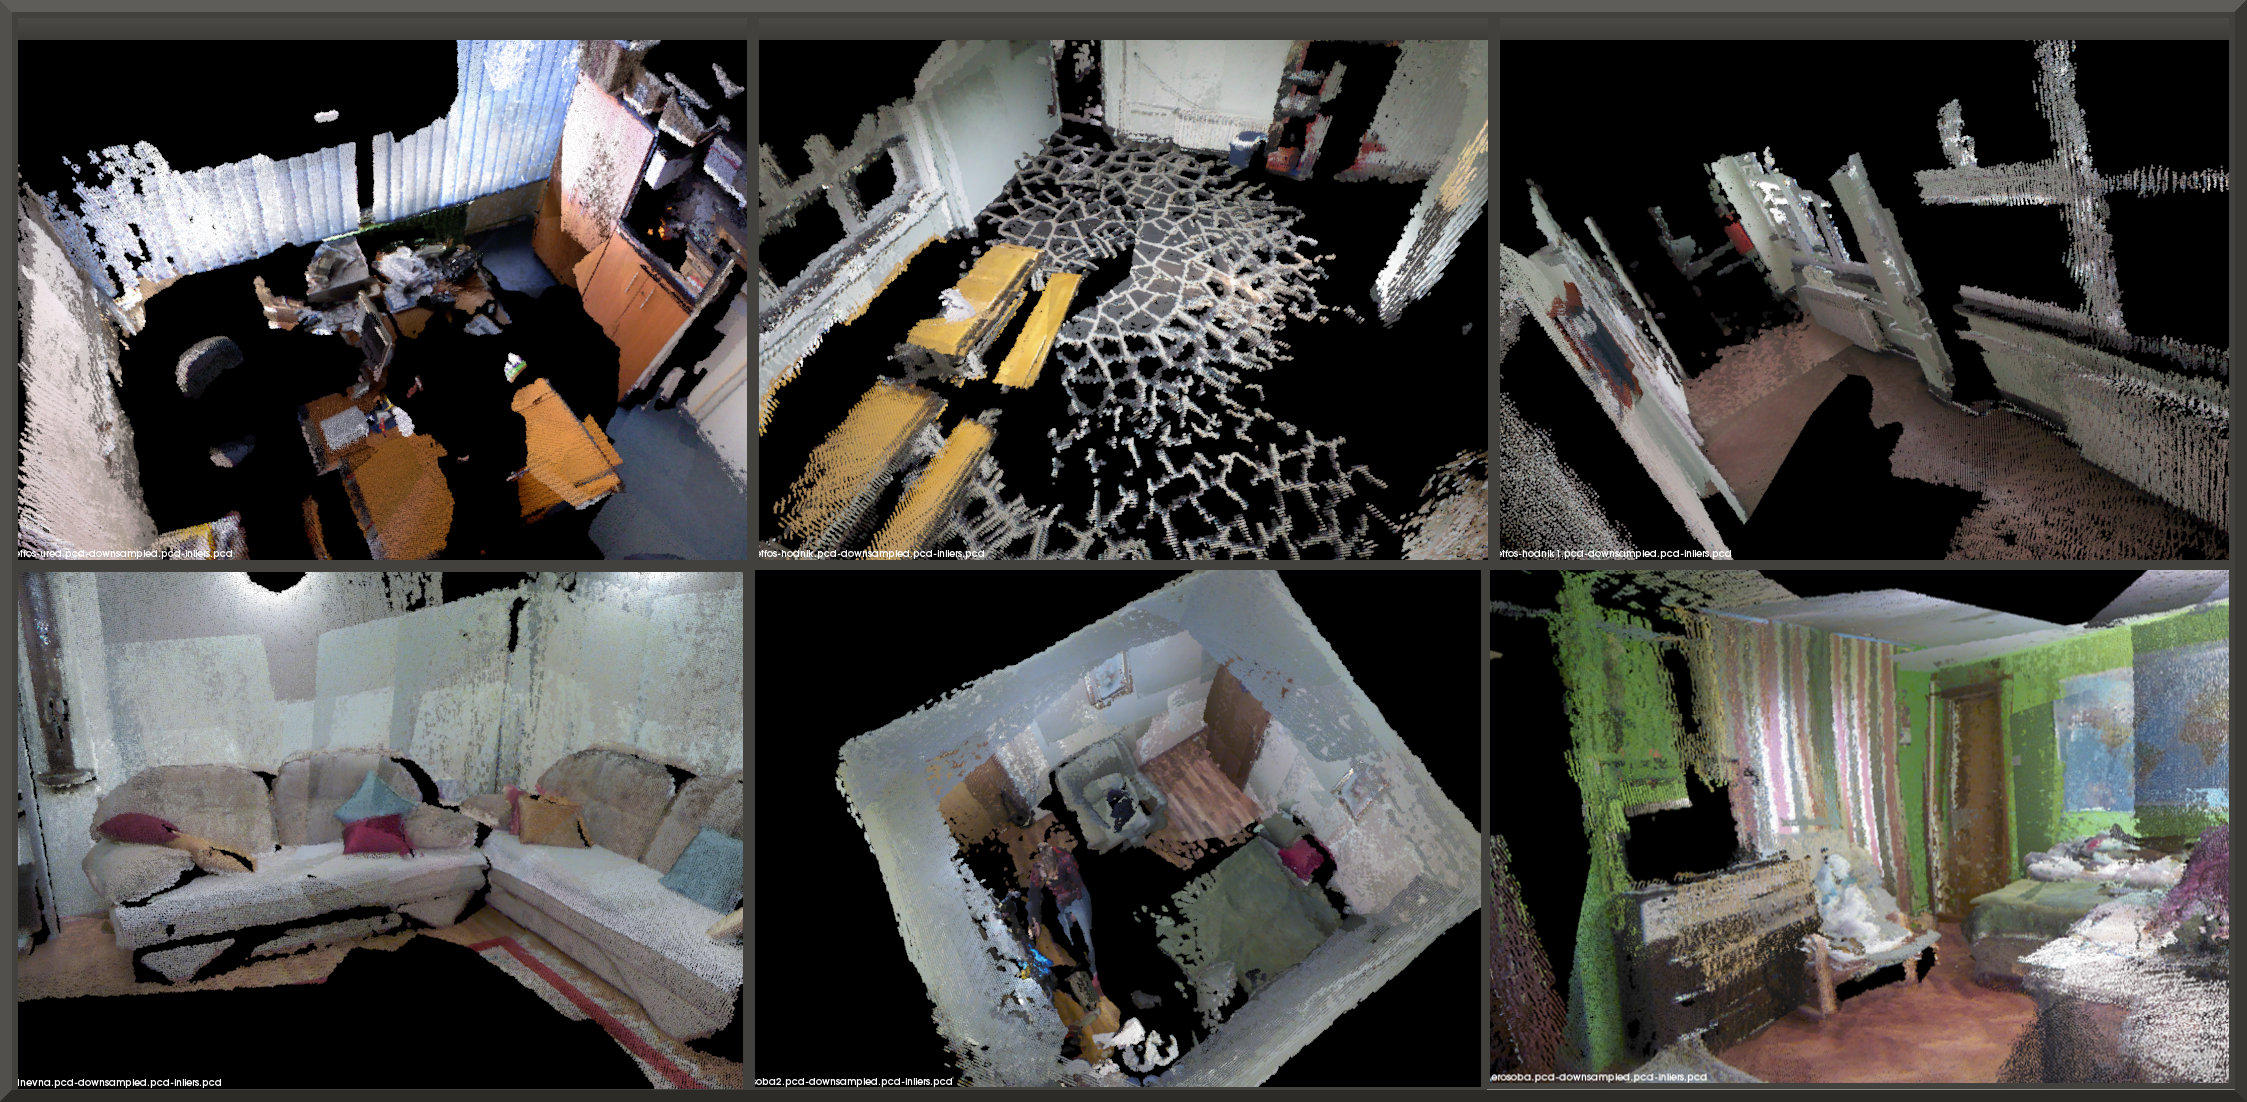
\includegraphics[scale=0.15]{figures/01-all-pcd.png}
\caption{Prikaz svih snimljenih scena}
\label{fig:01-all.png}
\end{figure}

\newpage
\subsection{Prikaz izgrađenih modela scena i objekata} % (fold)
\label{sub:Prikaz izgradenih modela scena i objekata}

\textbf{Snimka: Etfos ured 2013-07-30} 

\begin{figure}[h]
\centering
\includegraphics[scale=0.25]{figures/02-etfos-ured-vtk-pcd-all.png}
\caption{Prikaz izrađenog modela i snimljenog oblaka točaka}
\label{fig:02-etfos-ured-vtk-pcd.png}
\end{figure}

% subsection Prikaz izgrađenih modela scena i objekata (end)

% section Rezultati (end)


\newpage
\setcounter{figure}{0}

\section{Zaključak} % (fold)
\label{sec:Zaključak}

U ovom diplomskom radu razvijen je i predstavljen program za izgradnju
mreže trokuta mesh-reconstruction. Program se upotrebljava nad oblakom
točaka prikupljenim RGBDSlam programom. Ispitana je funkcionalnost i
kvaliteta postupka snimanjem i izgradnjom nekoliko 3D modela scena
pomoću 3D kamere. Tijekom izrade rada pojavilo se niz prepreka koje je
trebalo riješiti da bi se došlo do upotrebljivog programa. Glavne
prepreke su bile prevođenje, instalacija, proučavanje i pokretanja
programa RGBDSlam te postavljanje radne okoline za pisanje programa. 

Predstavljeni postupak snimanja i izgradnje 3D modela ima svoje
prednosti i nedostatke. Nedostatci su vezani uz ograničenja korištenih
tehnologija i algoritama. Npr. snimanje Kinectom ograničeno je na
prostore u unutrašnjosti, uspješnost snimanja RGBDSlam programom uvelike
ovisi o detekciji i sparivanju značajki, Poisson algoritam ne uzima u
obzir informaciju o boji itd. Prednosti je svakako nabavna cijena
kamere koja se može nabaviti za manje od tisuću kuna. Isto tako svi
korišteni programi objavljeni su pod slobodnim licencama te su dostupni
za proučavanje, poboljšavanje i upotrebu u bilo koje svrhe.  

Postoji potencijal opisanog postupka izgradnje odnosno generalna ideja
ima značajne mogućnosti buduće primjene. Sve veća dostupnost 3D printera 
na tržištu stvara potražnju za jednostavnim i jeftinim
rješenjem skeniranja 3D scena i objekata. Osim toga dizajneri FPS (engl.
\textit{First Person Shooter}) igara mogli bi koristiti sličan postupak
za skeniranje prostorija od kojih bi izgrađivali 3D modele.

Mogućnosti za poboljšanja postoje na svim razinama. Najveći utjecaj na
krajnje rezultate bilo bi proširivanje Poisson algoritma logikom za
očuvanje informacije o boji. Isto tako algoritamu bi se mogla dodati
logika koja uklanja zatvaranje velikih rupa, ideja je da se prođe još
jednom kroz izrađenu mrežu te pronađu i odbace veliki trokuti. Kod
snimanja scene jednostavno poboljšanje bilo bi korištenje jačeg računala
i automatskog snimanja. Najzahtjevniji je, mehanizam zatvaranja petlje o
kojemu značajno ovisi kvaliteta rezultata. To je još uvijek predmet
intenzivnog istraživanja. 

% section Zaključak (end)

\newpage
% Removing page numbering from this page but not from showing up on TOC
\thispagestyle{empty}
\begin{thebibliography}{9}

\bibitem{lamport94}
  Leslie Lamport,
  \emph{\LaTeX: A Document Preparation System}.
  Addison Wesley, Massachusetts,
  2nd Edition,
  1994.

\end{thebibliography}

\newpage

\section{Sažetak} % (fold)
\label{sec:Sažetak}

% section Sažetak (end)

\newpage

\section*{Životopis} % (fold)
\addcontentsline{toc}{section}{Životopis}
\label{sec:Životopis}

% section Životopis (end)

\newpage
\thispagestyle{empty}

\section*{Prilozi} % (fold)
\addcontentsline{toc}{section}{Prilozi}
\label{sec:Prilozi}

\subsection*{Prevođenje i instalacija RGBDSlam programa} % (fold)
\label{sub:RGBDSlam prilog}

Prevođenje i instalacije programa rađena je na Ubuntu 12.04 GNU/Linux
distribuciji pomoću skripte prikazane u ispisu~\ref{skripta} Upute za
ostale distribucije se nalaze na \url{http://wiki.ros.org/rgbdslam}.
Skripta automatizira dodavanje ROS repozitorija i poziva instalaciju
svih potrebinh paketa. Zatim postvlja ROS varijable okruženja potrebne za
pokretanje RGBDSlam programa. Tada se klonira izvorni kod programa i
pozivaju naredbe za instaliranje i prevođenje programa.

\begin{lstlisting}[language=bash,label=skripta, keywords={sudo, wget, 
    echo, apt-get, rosdep, roscd, rosmake}, caption={Ispis shell skripte 
    za instalaciju rgbdslam programa}]
# Better pick a mirror close to you. 
# See http://ros.org/wiki/ROS/Installation/UbuntuMirrors
sudo sh -c '. /etc/lsb-release && echo "deb http://packages.ros.org/ros/ubuntu $DISTRIB_CODENAME main" > /etc/apt/sources.list.d/ros-latest.list' 

wget http://packages.ros.org/ros.key -O - | sudo apt-key add -

sudo aptitude update

# This will draw gigabytes from the network:
sudo apt-get install ros-fuerte-perception-pcl ros-fuerte-vision-opencv ros-fuerte-octomap-mapping python-rosdep 
sudo apt-get install ros-fuerte-openni-launch

echo 'source /opt/ros/fuerte/setup.bash' >> ~/.bashrc
echo 'export ROS_PACKAGE_PATH=~/ros:$ROS_PACKAGE_PATH' >> ~/.bashrc
. ~/.bashrc

svn co http://alufr-ros-pkg.googlecode.com/svn/trunk/rgbdslam_freiburg ~/ros/rgbdslam_freiburg

sudo rosdep init
rosdep update
rosdep install rgbdslam_freiburg
roscd rgbdslam

# This will take a while:
rosmake rgbdslam_freiburg
\end{lstlisting}


% subsection RGBDSlam prilog (end)

% section Prilozi (end)


\end{document}
